%% -----------------------------------------------------------------------------
% \subsection{Contextualizing the results through an example scenario}

\begin{figure}
{
  \definecolor{trans-fb}{RGB}{215, 48, 31}
  \definecolor{trans-lb}{RGB}{252, 141, 89}
  \definecolor{trans-exn}{RGB}{253, 204, 0}
  \definecolor{erasure}{RGB}{119, 87, 254}

  \newcommand\config[1]{\begin{minipage}{0.09\textwidth}\centering\includegraphics[width=\linewidth]{Images/#1}\end{minipage}}
  \newcommand\runtimeError{\begin{minipage}{0.03\textwidth}\centering
\includegraphics[width=\linewidth]{Images/runtime-error}\end{minipage}}
  \newcommand\checkFailure{\begin{minipage}{0.03\textwidth}\centering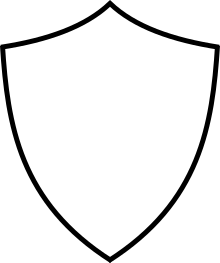
\includegraphics[width=\linewidth]{Images/check-failure-plain}\end{minipage}}
  \newcommand\blameFinger{\begin{minipage}{0.02\textwidth}\centering\vspace{0.25em}\includegraphics[width=\linewidth]{Images/finger}\end{minipage}}
  \newcommand\typeError{\scalebox{1.5}{$\tau_{\hspace{-0.1em}\times}$}}
  \newcommand\success{\textcolor{black!30!green}{\checkmark}}
  \newcommand\fail{\textcolor{red}{\sffamily x}}
  \footnotesize
\centering
\begin{tabular}{l|ccl|ccl|cc|c}
\multicolumn{3}{c}{\begin{minipage}{0.25\textwidth}\centering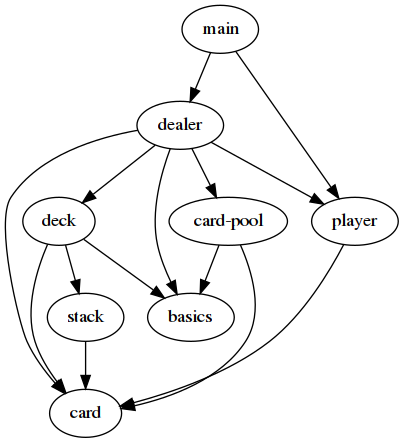
\includegraphics[width=\linewidth]{Images/take5-module-graph}\end{minipage}} &
\multicolumn{7}{c}{\begin{minipage}{0.69\textwidth}\centering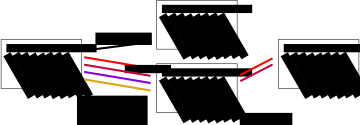
\includegraphics[width=\linewidth]{Images/trails-example}\end{minipage}} \\
\multicolumn{3}{c}{\begin{minipage}{0.25\textwidth}\centering the dependency graph\end{minipage}} &
\multicolumn{7}{c}{\begin{minipage}{0.69\textwidth}\centering the paths taken by each mode through the configuration lattice\end{minipage}} 
\vspace{1em} \\
\end{tabular}

\begin{tabular}{l|ccl|ccl|cc|c}
 & \textbf{Root} &  &  & \textbf{Step 1} &  &  & \textbf{Step 2} &  & \textbf{Success?}\\
\textbf{Mode} & config & result & stack & config & result & stack & config & result & \\
\hline
Natural & \config{10001100} & \blameFinger & \texttt{main} & \config{10001110} & \typeError &  &  &  & \success\\
-blame &  & \texttt{player} & \texttt{main} &  &  &  &  &  & \\
\hline
\textcolor{trans-fb}{Transient} & \config{10001100} & \runtimeError & \texttt{dealer} & \config{10011100} & \blameFinger & \texttt{dealer} & \config{10011110} & \typeError & \success\\
\textcolor{trans-fb}{-first-blame} &  &  & \texttt{dealer} &  & \texttt{player} &  &  &  & \\
\emph{and} &  &  & \texttt{dealer} &  & \texttt{dealer} &  &  &  & \\
\textcolor{trans-lb}{-last-blame} &  &  & \texttt{main} &  &  &  &  &  & \\
\hline
\textcolor{erasure}{Erasure} & \config{10001100} & \runtimeError & \texttt{dealer} & \config{10011100} & \runtimeError & \texttt{dealer} &  &  & \fail\\
 &  &  & \texttt{dealer} &  &  & \texttt{dealer} &  &  & \\
 &  &  & \texttt{dealer} &  &  & \texttt{dealer} &  &  & \\
 &  &  & \texttt{main} &  &  & \texttt{main} &  &  & \\
\hline
\textcolor{gray}{Natural} & \config{10001100} & \checkFailure & \texttt{main} &  &  &  &  &  & \fail\\
\textcolor{gray}{-exceptions} &  &  & \texttt{main} &  &  &  &  &  & \\
\hline
\textcolor{trans-exn}{Transient} & \config{10001100} & \runtimeError & \texttt{dealer} & \config{10011100} & \checkFailure & \texttt{dealer} &  &  & \fail\\
\textcolor{trans-exn}{-exceptions} &  &  & \texttt{dealer} &  &  &  &  &  & \\
 &  &  & \texttt{dealer} &  &  &  &  &  & \\
 &  &  & \texttt{main} &  &  &  &  &  & \\
\end{tabular}

\begin{minipage}{0.95\textwidth}
\vspace{0.5em}
\centerline{\it Legend}

\noindent{\bf config} Each box corresponds to a module and indicates (with x) if it is typed. 
The mutated module is gray.

\medskip

\noindent{\bf result}\\
\begin{center}
\begin{tabular}{l@{\quad}l}
symbol        & denotation \\ \hline 
\blameFinger  & the configuration results in a dynamic type-check failure, blaming the module(s) below \\
\typeError    & the configuration does not type check\\
\runtimeError & the configuration fails a check to the runtime system\\
\checkFailure & the configuration signals a dynamic type check failure for which blame is ignored\\
\end{tabular}
\end{center}

\end{minipage}}


\caption{An example scenario from take5, with every mode's resulting trail.}
\label{fig:example-trails}
\end{figure}

Interpreting the numeric summaries and aggregations of the last section demands an intuitive understanding of what blame trails look like in practice.
Thus, before drawing high level conclusions, let us examine one set of scenarios with a typical debugging scenario from the {\tt take5} benchmark,
whose module dependency graph is shown in the top left of figure~\ref{fig:example-trails}.

The rest of figure~\ref{fig:example-trails} illustrates the blame trails produced by every mode of the rational programmer for the debugging scenario in
two different ways: 
\begin{itemize}

\item The top right shows the blame trails produced by every mode of the rational programmer as paths through the configuration lattice starting at the
root (leftmost) configuration. Each configuration is represented by a bit string where each digit corresponds to a module in the program and indicates if
it is typed.

\item The table in the middle expands the information in the diagram with the details of every step in each trail.
Every row of the table represents the trail of one mode. The middle-three columns depict the steps of a blame trail:
\begin{description}
\item[Root] describes the result of running the root configuration in this row's mode.
\item[Step 1] is the result of the rational programmer's reaction to the outcome of running the root. 
\item[Step 2] shows the result of reacting to the outcome of running step~1 configuration, if any. 
\end{description}
Finally, the \textbf{Success?} column summarizes whether exploring the trail succeeds.

\end{itemize}

Let us contrast rows 1 and~4. The first one shows that running the root
configuration under the Natural-blame mode fails due a dynamic type check and
blames the {\tt player} module; typing that module and running again then
results in a type error, and hence the trail is successful.  By contrast, the
Natural-exceptions mode (row 4) yields stack information for the root
configuration that is unhelpful; it identifies only {\tt main}, which is already
typed. Hence, this trail immediately gets stuck.

In short, this figure concretely demonstrates how the rational programmer
behaves in different modes. In this case, the behaviors differ from each other
in all five modes. The reader may keep these scenarios in mind as we next
discuss the numeric results of the last section.

\subsection{Interpreting the results}

The results of the experiment suggests a number of high-level conclusions about
blame strategies in the gradual typed world.  First, run-time type checks have a
large positive impact, regardless of whether these checks assign blame or throw
plain exceptions.  Second, error messages with blame assignments are more
helpful than those without. The results also indicate, though, that blame is not
critical in a majority of cases, and therefore they suggest investigating
whether blame tracking is worth the performance cost.  Third, the Natural
approach fares better than the Transient approach, but only by a small margin.
Since Natural offers complete and sound path-based blame (i.e. it blames all and only those components
that are relevant to a type impedance mismatch) while Transient offers
incomplete but sound heap-based blame~\citep{gfd-oopsla-2019}, the results call
for a study concerning the relative strengths of the two models of blame.
Fourth, given that Transient's sound but shallow run-time type checks do not
seem to hamper debugging, a version of the Natural semantics of Typed Racket
that disables some of its wrappers may offer an answer to the well-known
performance issues of Natural~\citep{gtnffvf-jfp-2019}.  Fifth, given that both
modes of the Transient rational programmer are equally successful and that
Transient-last produces shorter trails, Reticulated Python could limit the size
of blame sequences to the last few entries to reduce its serious performance
problems (see below).

The validity of these conclusions is threatened in several ways: (i) the
representativeness of benchmarks; (ii) the relation between mutations and real
programming mistakes; (iii) the definition of interesting debugging scenarios;
and (iv) the sampling strategy. While these threats have been mitigated by the
experimental setup, the remainder of this section discusses three additional
ones.

%% -----------------------------------------------------------------------------
\subsection{Threat: Is the Rational Programmer Realistic?}

Like {\em homo economicus\/}, which decouples the actual behavior of a
participant in an economy for the sake of mathematical modeling, the model of a
rational programmer decouples the actual debugging behavior of a software
developer for the sake of a systematic, large-scale analysis. This decoupling
comes with advantages and disadvantages. In the economic realm, mathematical
models have provided some predictive insights into the market's behavior; but as
behavioral economics has shown more recently (e.g.~\cite{henrich2001search}), the mathematical abstraction of a
rational actor makes predictions also quite unreliable in some situations.
\footnote{It has misled economists to focus on just mathematics, though
this problem is not relevant here---tongue firmly in cheek.}  Just like an
ordinary consumer or producer, an actual software developer is unlikely to stick
to the exact strategy proposed here. When this happens, the predicted benefits
of blame assignment may not materialize. Indeed, the authors' personal
experience suggests such deviations, and it also suggests that deviating often leads to dead-ends.
To make a true judgment of the usefulness of the rational-programmer
idea, the community will need much more experience with this form of evaluation
and relating the evaluation to the behavior of working programmers.

Relatedly, the experimental setup hides how a rational programmer ascribes types
to extend a trail. When the run-time checks signal an impedance mismatch in the
real world, a real-world programmer does not have a typed module ready to swap
in. Instead, the programmer must come up with the next set of types, which means
making choices. It is usually possible to consistently assign types to variables
in a module in different ways. The maintenance of the benchmarks over many years
has driven home this lesson but, fortunately, it has also shown that the types
are in somewhat canonical.  The authors therefore conjecture that different
real-world programmers would often come up with equivalent type assignments
during debugging sessions. 

%% -----------------------------------------------------------------------------
\subsection{Threat: Why Does Transient Lose Blame?} \label{sec:threat:transient}

The execution of the experiment reveals that Transient produces empty blame
sequences for 967 scenarios. In theory, empty set must not occur. An empty blame
sequence means a lack of boundary crossings for the witness value.  By
implication, a typed module is blaming itself---something that can happen only
if the type checker (or system) is unsound.

An investigation of these empty blame cases reveals that Transient is not
unsound but that Vitousek et al.'s Transient blame assignment loses track
of the proper boundaries due to an incomplete initialization of the blame map.
Despite these losses, the number of failures is a small fraction of the
overall number of debugging scenarios. It is unlikely that any
improvements to Vitousek et al.'s strategy would change the overall
conclusion about Transient blame.

{\bf Note} The scenarios where Transient returns no blame suggest two ways to
improve its blame map.  First, entries in a blame map should point to {\em
several\/} parent entries.  For example, if \texttt{f} receives bad input in the
context of {\tt (filter f xs)}, the entry should point to both \texttt{filter}
and \texttt{xs}. Second, the construction of entries must be guided by type-like
specifications for primitives instead of special cases for built-in
functions. Aliasing such function changes the blame map.  


%% -----------------------------------------------------------------------------
\subsection{Threat: Is the Transient Blame Assignment Mechanism Realistic?}
\label{sec:threat:transient2}

The results in section~\ref{sec:results} also show that the cost of Transient
blame is quite high. Under the Transient semantics, some of the debugging
scenarios exceed the 4-minute timeout or the 6GB-memory limit. To put those
limits into context, the fully typed and fully untyped benchmarks all normally complete
in a few seconds with minimal memory usage. Furthermore, none of the mixed
Natural configurations hit these limits, and with the blame map turned off,
the Transient semantics also runs these programs in a short amount of time and
well within the memory limits. In short, even though the Transient rational
programmer appears to do well in the experiment, the implementation of the
Transient blame strategy might be unrealistic. 

At first glance, these measurements seem to contradict the results
of~\citet{vss-popl-2017}. They report an average slowdown of 2.5x and a
worst-case of 5.4x on the fully-typed Python benchmarks in Reticulated Python.
Unfortunately, the high cost of Shallow Racket seems closer to the truth.
There are at least four broad issues that skew the earlier results:
\begin{enumerate}

\item The 2017 implementation of Reticulated fails to insert certain soundness
checks\footnote{Missing check:
\url{https://github.com/mvitousek/reticulated/issues/36}} and blame-map
updates\footnote{Missing cast:
\url{https://github.com/mvitousek/reticulated/issues/43}} from the paper.

\item The types of almost all local variables in the "fully typed" benchmarks is
{\tt Dynamic}, often due the impoverished nature of the type system, which does
not allow the ascription of precise types.  Code that ends up with the type {\tt
Dynamic} has fewer constraints to check at run-time---and much less information
to track in the blame map.

\item \citet{vss-popl-2017} use small benchmarks.  Four have since been retired
from the official Python benchmark suite because they are too small,
unrealistic, and unstable.\footnote{Release notes:
\url{https://pyperformance.readthedocs.io/changelog.html}}

\item On non-trivial programs, Reticulated Python suffers from the same high
overhead as Shallow Racket.  It runs the simplest benchmark from the GTP suite (translated into Python)
in approximately 40 seconds without blame and times out after 10 minutes when
the blame map is enabled.

\end{enumerate}
More work on Transient blame is needed to make an informed decision. 


%% NOTE: Vitousek's benchmarks are from the Python "pyperformance" suite.
%%   The version notes in the docs talk about retiring benchmarks, but
%%   you can also look at the current codebase and see what names from POPL'17
%%   are missing: callsimple, callmethod, callmethodslots, & pystone
%% <https://github.com/python/pyperformance/tree/master/pyperformance/benchmarks>
